\documentclass{ctexrep}
\usepackage[margin=25mm]{geometry}
\usepackage{amsmath}
\usepackage{fancyhdr}
\usepackage{cite}
\usepackage{graphicx}
\usepackage{float}
\usepackage{indentfirst}
\usepackage[utf8]{inputenc}
\usepackage{amssymb}
\usepackage{hyperref}


\usepackage{titlepic}
\providecommand{\keywords}[1]
{
  \small	
  \textbf{\textit{关键词}} #1
}










%\usepackage[linesnumbered,boxed]{algorithm2e}
\usepackage{listings}
\usepackage{xcolor}

\definecolor{codegreen}{rgb}{0,0.6,0}
\definecolor{codegray}{rgb}{0.5,0.5,0.5}
\definecolor{codepurple}{rgb}{0.58,0,0.82}
\definecolor{backcolour}{rgb}{0.95,0.95,0.92}

\lstdefinestyle{mystyle}{
    backgroundcolor=\color{backcolour},   
    commentstyle=\color{codegreen},
    keywordstyle=\color{magenta},
    numberstyle=\tiny\color{codegray},
    stringstyle=\color{codepurple},
    basicstyle=\ttfamily\footnotesize,
    breakatwhitespace=false,         
    breaklines=true,                 
    captionpos=b,                    
    keepspaces=true,                 
    numbers=left,                    
    numbersep=5pt,                  
    showspaces=false,                
    showstringspaces=false,
    showtabs=false,                  
    tabsize=2
}

\lstset{style=mystyle}


\pagestyle{fancy}
\chead{不围棋博弈}


\begin{titlepage}
    \titlepic{
\includegraphics[width=0.4\textwidth]{9.jpg}}
    
    \title{2021年春季学期
数据结构课程设计A2题实验报告
}
    \author{软件学院19级
    
    8班张津赫}
    \date{April 2021}

    
    
    
\end{titlepage}


\begin{document}
\maketitle

\begingroup
    \fontsize{14pt}{16pt}\selectfont
      
       
    
\begin{abstract}
     \hspace{1cm}本题使用了蒙特卡洛树搜索即MCTS的方法,蒙特卡洛树搜索MCTS是一种针对决策类博弈游戏,运用蒙特卡洛模拟方法进行评估博弈策略的启发式
搜索算法。
     MCTS的重点是对最有前途的举动进行分析,并基于对搜索空间的随机采样来扩展搜索树。在每次模拟(roll-out)时,通过随机选择移动来将游戏进行到最后。然后将每次roll-out的最终游戏结果用于对游戏树中的节点进行加权,以便在将来的roll-out中更有可能选择更好的节点。
每一轮蒙特卡洛树搜索均包含四个步骤: 选择 \hspace{0.3cm}扩展\hspace{0.3cm} 模拟 \hspace{0.3cm}反向传播

\vspace{1cm}\hspace{0.3cm}\keywords{\large(MCTS,启发式算法,UCB,AlphaGo)}



\end{abstract}

\endgroup



\maketitle  % 生成 Summary Sheet
\tableofcontents  % 生成目录
\chapter{算法思想}
\section{总体思路}
采用了Monte Carlo Tree Search方法 
MCTS使用蒙特卡洛模拟来积累价值估算,以指导搜索树中高回报的轨迹。MCTS更加关注更有前途的节点,因此避免了强行使用所有不切实际的可能性的情况。
MCTS的核心是重复的迭代(理想情况下是无限的,实际上受计算时间和资源的限制),该迭代包括 四个步骤: 选择 扩展 模拟 反向传播


UCT是一个让我们从已访问的节点中选择下一个节点来进行遍历的函数,也是MCTS的核心函数


\begin{equation}\label{eq:eq1}
\underset{v^{\prime} \in \text { children of } v}{\arg \max } \frac{Q\left(v^{\prime}\right)}{N\left(v^{\prime}\right)}+c \sqrt{\frac{2 \ln N(v)}{N\left(v^{\prime}\right)}}\end{equation}





其中v'表示当前树节点,v表示父节点,Q表示这个树节点的累计quality值,N表示这个树节点的visit次数,C是一个常量参数(可以控制exploitation和exploration权重)。
这个公式的意思时,对每一个节点求一个值用于后面的选择,这个值有两部分组成,左边是这个节点的平均收益值(越高表示这个节点期望收益好,越值得选择,用于exploitation),右边的变量是这个父节点的总访问次数除以子节点的访问次数(如果子节点访问次数越少则值越大,越值得选择,用户exploration),因此使用这个公式是可以兼顾探索和利用的。
\begin{itemize}

\item 选择(Selection)

即找一个最好的值得探索的结点,通常是先选择没有探索过的结点,如果都探索过了,再选择UCB值最大的进行选择(UCB是由一系列算法计算得到的值,这里先不详细讲,可以简单视为value)

\item 扩展(Expansion)

已经选择好了需要进行扩展的结点,那么就对其进行扩展,即对其一个子节点最为下一步棋的假设,一般为随机取一个可选的节点进行扩展。

\item 模拟(Simulation)

扩展出了子节点,就可以根据该子节点继续进行模拟了,我们随机选择一个可选的位置作为模拟下一步的落子,将其作为子节点,然后依据该子节点,继续寻找可选的位置作为子节点,依次类推,直到博弈已经判断出了胜负,将胜负信息作为最终得分。

\item 回溯更新(Backpropagation)

将最终的得分累加到父节点,不断从下向上累加更新。

\end{itemize}
\thispagestyle{empty}
\section{所用方法的特别、新颖或创新之处}
通过不断地测试调参,最终找到了对运算结果最好的时间范围,和使ucb的值更有价值的系数c的最佳值0.2。

\begin{lstlisting}[language=C++]
int timeout = (int)((0.9765) * (double)CLOCKS_PER_SEC); 

double score = p->number_of_wins / (p->number_of_simulations) + 0.2 * C * sqrt(log(2 * number_of_simulations) / (p->number_of_simulations));

\end{lstlisting}





\section{算法流程图}


\begin{figure}[h] %figure环境,h默认参数是可以浮动,不是固定在当前位置。如果要不浮动,你就可以使用大写float宏包的H参数,固定图片在当前位置,禁止浮动。
    \centering %使图片居中显示
    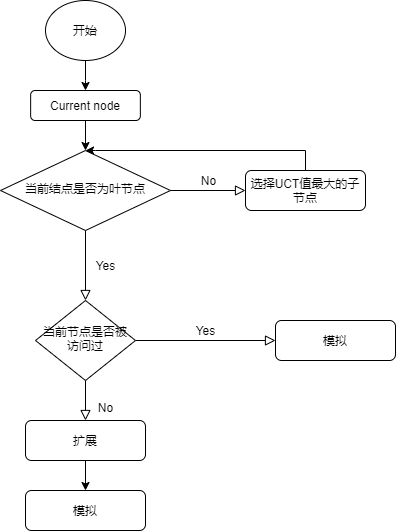
\includegraphics[width=0.6\textwidth]{mcts.png} %中括号中的参数是设置图片充满文档的大小,你也可以使用小数来缩小图片的尺寸。
    \caption{流程图1} %caption是用来给图片加上图题的
    \label{wolf} %这是添加标签,方便在文章中引用图片。
\end{figure}%figure环境



\begin{figure}[H] %figure环境,h默认参数是可以浮动,不是固定在当前位置。如果要不浮动,你就可以使用大写float宏包的H参数,固定图片在当前位置,禁止浮动。
    \centering %使图片居中显示
    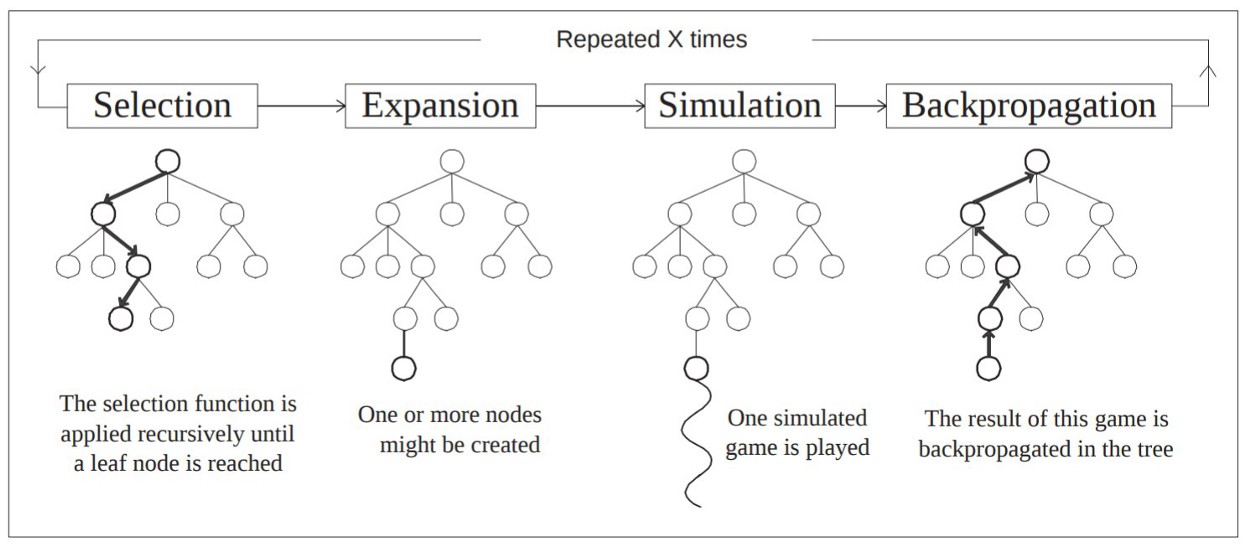
\includegraphics[width=1\textwidth]{sss.jpeg} %中括号中的参数是设置图片充满文档的大小,你也可以使用小数来缩小图片的尺寸。
    \caption{流程图2} %caption是用来给图片加上图题的
    \label{wolf} %这是添加标签,方便在文章中引用图片。
\end{figure}%figure环境




\section{算法运行时间复杂度分析}
时间复杂度为
\begin{equation}\label{eq:eq1}
\mathrm{O}(\mathrm{mkI} / \mathrm{C}) \mathrm{m}\end{equation}


m代表每次搜索,随机选择的子节点数量
k 代表每次并行搜索的数量 本程序中为1,
I代表迭代次数,
C表示可用核心数量
		


程序中
\begin{lstlisting}[language=C++]
    MCTS_Node::dfsAir(int fx, int fy)
\end{lstlisting}

时间开销大,而且会被调用很多次,若对此算法进行改进,将会大幅提升速度,以进行更多次的模拟。

\chapter{程序代码说明}


\section{数据结构说明}
运用了树型结构
\begin{lstlisting}[language=C++]
   

class MCTS_Node
{
public:
    MCTS_Node();
    
    int Max_Childen = 0; //最大可有的孩子节点数量
    
    int Number_of_Children = 0;//记录现有几个孩子节点
    
    MCTS_Node *children[81];

    int current_board[9][9] = {0};

    int col = 0;//表示黑旗还是白旗
    
    MCTS_Node *parent = NULL;
   
    int number_of_simulations = 0;
    
    double number_of_wins = 0.00;
    
    int available_position[81];//棋盘上可以下的位置
    
    void get_available_position(); //得到可以落子的位置
    
    bool dfsAir(int fx, int fy);         //判断是否有气
    
    bool judgeAvailable(int fx, int fy); //判断是否可下 只判断 不改变
    
    double roll_out();   //模拟
    
    MCTS_Node *Selection(double C);  
    
    MCTS_Node *Expansion();
    
    MCTS_Node *tree_search_process();
    
    void Backpropagation(double reward);
};


\end{lstlisting}

\section{函数说明}

\begin{lstlisting}[language=C++]
void get_available_position();

bool dfsAir(int fx, int fy);

bool judgeAvailable(int fx, int fy);

double roll_out();

MCTS_Node *Selection(double C);  

MCTS_Node *Expansion();

MCTS_Node*tree_search_process();

void Backpropagation(double reward);
\end{lstlisting}
\section{程序限制}
在面对专业玩家或者更高级的机器人时,因为在模拟时是随机搜索,所以可能存在单个分支没有被“看到”,导致失败。

纯粹的随机掷点可以保证良好的随机性,但 是 随 机 性 很
强会影响到做出正确评估的收敛速度,尤其是对于类似于围
棋的决策游戏,状态空间非常庞大,本身能探索到的空间只是
一个小的部分,太强的随机性反而会使很多资源浪费到不必
要考虑的状态空间中。

\chapter{实验结果}



\section{测试数据}
在botzone上进行了大量对抗训练


\section{结果分析}
蒙特卡洛算法在步数较少时不敌估值函数,但随着步数的增加,MCTS的优势便显现了出来。
在面对随机策略以及低级别玩家时,MCTS具有压倒性的优势,对于同样使用MCTS方法的对手,输赢很大程度上取决于谁的模拟次数更多,所以尽可能多的优化程序,压缩时间是必要的。但在面对某些针对不围棋特定研发的巧妙的价值评估程序时,MCTS反而占不到便宜,甚至会输掉。
\section{经典战局}
\begin{figure}[H] %figure环境,h默认参数是可以浮动,不是固定在当前位置。如果要不浮动,你就可以使用大写float宏包的H参数,固定图片在当前位置,禁止浮动。
    \centering %使图片居中显示
    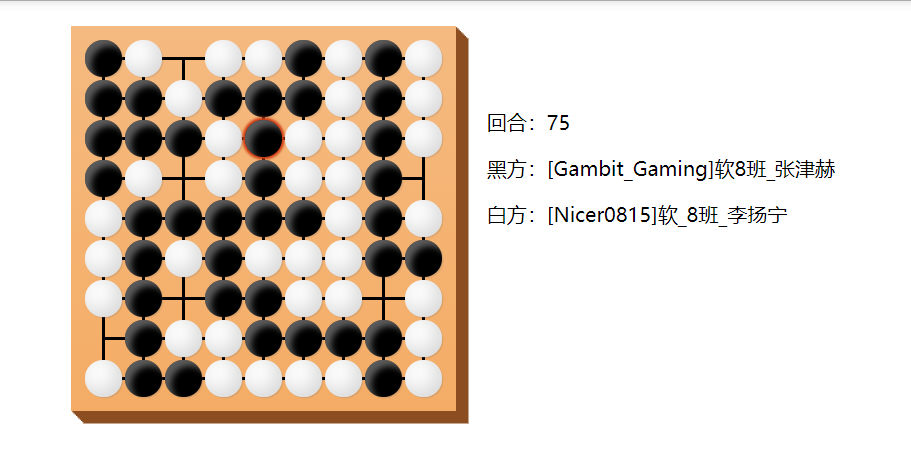
\includegraphics[width=0.8\textwidth]{1.png} %中括号中的参数是设置图片充满文档的大小,你也可以使用小数来缩小图片的尺寸。
    \caption{MCTS对阵MCTS胜利} %caption是用来给图片加上图题的
    \label{wolf} %这是添加标签,方便在文章中引用图片。
\end{figure}%figure环境



\begin{figure}[H] %figure环境,h默认参数是可以浮动,不是固定在当前位置。如果要不浮动,你就可以使用大写float宏包的H参数,固定图片在当前位置,禁止浮动。
    \centering %使图片居中显示
    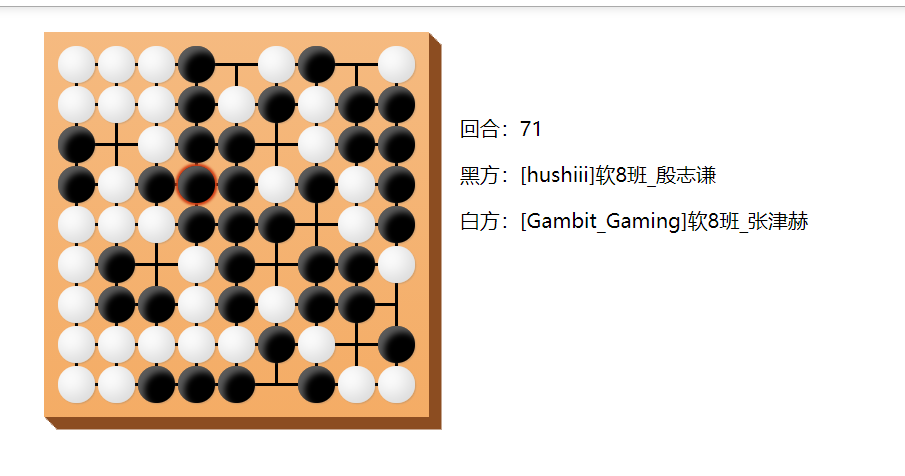
\includegraphics[width=0.8\textwidth]{2.png} %中括号中的参数是设置图片充满文档的大小,你也可以使用小数来缩小图片的尺寸。
    \caption{MCTS对阵价值评估失利} %caption是用来给图片加上图题的
    \label{wolf} %这是添加标签,方便在文章中引用图片。
\end{figure}%figure环境











{\let\clearpage\relax\chapter*{总结}}
%\chapter{总结}
蒙特卡洛树搜索是一种广泛运用于强化学习的决策方
法, 它的本质在于从当前的根结点下的子节点中选择最优子
节点来作为决策的结果, 即采用一种贪心算法使每一步的累
积计分都达到最大,从而使得到最好的结果。 但是,蒙特卡洛
算法只能解决有限步数的问题,当问题步数太多或无限时,由
于迭代次数不允许,无法用蒙特卡洛算法来解决。 例如在解决
围棋问题时,由于围棋的状态空间太过庞大,利用暴力搜索的
方法无法穷尽。 所以只能使用经过改进的 Monte-Carlo 法,即
从给定落子位置开始,随机采样,得到一个模拟的结果。 经过
多次采样之后,将平均成功率返回作为该点的成功率。











在对阵同样使用MCTS的对手时,双方决定胜负在六十几局,而这时先手还是后手起到了一定的作用,一种解决方法是在simulation阶段,想出一种比对手更高效的方法,其一是使rollout过程更加快速,这样可以进行更多次搜索。其二是更精巧的计算reward值,使reward值在UCT值计算中更有效果。
\chapter{参考文献}


\begin{lstlisting}[language=java]
https://www.geeksforgeeks.org/ml-monte-carlo-tree-search-mcts/

https://www.wikiwand.com/en/Monte_Carlo_tree_search

https://medium.com/@quasimik/monte-carlo-tree-search-applied-to-letterpress-34f41c86e238

https://towardsdatascience.com/monte-carlo-tree-search-an-introduction-503d8c04e168

\end{lstlisting}
\bibliographystyle{plain}
\bibliography{ref}
\bibliography{Reference.bib}
  


\end{document}